\documentclass[11pt,a4paper]{article}
\usepackage[margin=1in]{geometry}
\usepackage{amsmath,amssymb}
\usepackage{graphicx}
\usepackage{subcaption}
\usepackage{booktabs}
\usepackage{fancyhdr}
\usepackage{enumitem}

\pagestyle{fancy}
\fancyhf{}
\lhead{Laboratory Report}
\rhead{AI5707: PRML -- Lab Assignment 5}
\cfoot{Page \thepage}
\renewcommand{\headrulewidth}{0.4pt}

\setlist[itemize]{itemsep=2pt,topsep=4pt}

\begin{document}

\begin{center}
{\LARGE \textbf{Maximum Likelihood Parameter Estimation and Bayes Decision Boundaries}}\\[8pt]
{\large Lab Assignment 5 Report}\\[8pt]
Shrawanthi P. (Roll No: 26120098)\\
Shreepriyadarshini RM. (Roll No: 26120099)\\[4pt]
5th October 2026
\end{center}

\section{Introduction and Objectives}
In this assignment, we use Maximum Likelihood Estimation (MLE) for parameter estimation of 2-D Gaussian distributions from generated and real-world data. We then classify the test data using the Bayes decision rule and analyze how different covariance matrix structures affect the shape and orientation of decision boundaries across all three classes.

The primary objectives are:
\begin{enumerate}
  \item Generate 10,000 2-D Gaussian data points for each of three classes $\mathcal{N}(\mu_i,\Sigma_i)$ ($i=1,2,3$).
  \item Implement and evaluate six different covariance configurations:
  \begin{itemize}
    \item Identical covariance across classes: (a) Isotropic ($\sigma^2 I$), (b) Diagonal, and (c) Full covariance.
    \item Different covariances across classes: (a) Isotropic, (b) Diagonal, and (c) Full covariance.
  \end{itemize}
  \item Split the synthetic dataset into 80\% training data (24,000 samples) and 20\% test data (6,000 samples).
  \item Estimate class parameters ($\hat{\mu}_i, \hat{\Sigma}_i, \hat{P}(\omega_i)$) using Maximum Likelihood Estimation.
  \item Classify the test data using the Bayes decision rule, compute test accuracy and confusion matrices, and plot decision boundaries with test data overlaid.
  \item Estimate class parameters for the given real-world dataset, classify test data, and plot decision boundaries.
  \item Plot ROC curves and evaluate AUC for all classification problems.
\end{enumerate}

\section{Experiments and Results}
The true class centers for the synthetic data are kept constant across all experiments:
\begin{equation}
\mu_1=\begin{bmatrix}-2.0\\0.0\end{bmatrix},\quad
\mu_2=\begin{bmatrix}2.0\\0.0\end{bmatrix},\quad
\mu_3=\begin{bmatrix}0.0\\3.0\end{bmatrix}
\end{equation}
For each class, 10,000 samples were generated (30,000 samples total). In every case, 80\% (24,000 samples) are used for training and 20\% (6,000 samples) for testing.

\subsection{Identical Covariance Across Classes}
In Cases 1, 2, and 3, all three classes have the same covariance matrix. As shown in Figure~\ref{fig:identical}, all decision boundaries are piecewise straight lines. The corresponding one-vs-rest ROC curves are shown in Figure~\ref{fig:identical_roc}.

\begin{figure}[ht]
\centering
\begin{subfigure}{0.32\textwidth}
  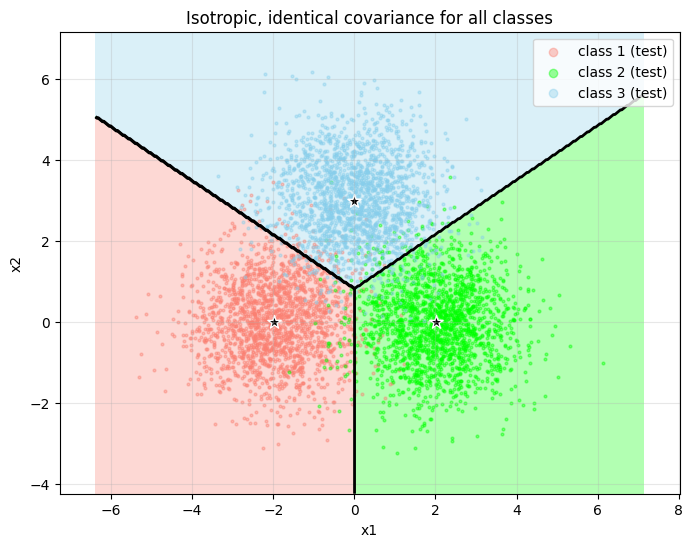
\includegraphics[width=\textwidth]{case1.png}
  \caption{Case 1: Isotropic shared}
\end{subfigure}\hfill
\begin{subfigure}{0.32\textwidth}
  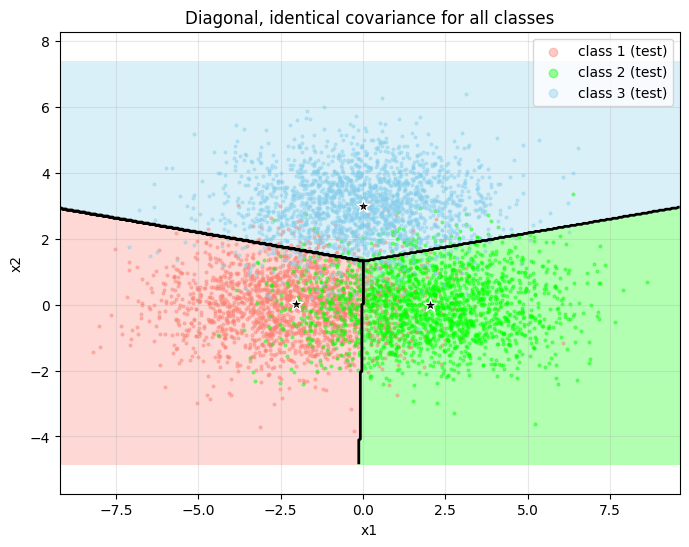
\includegraphics[width=\textwidth]{case2.png}
  \caption{Case 2: Diagonal shared}
\end{subfigure}\hfill
\begin{subfigure}{0.32\textwidth}
  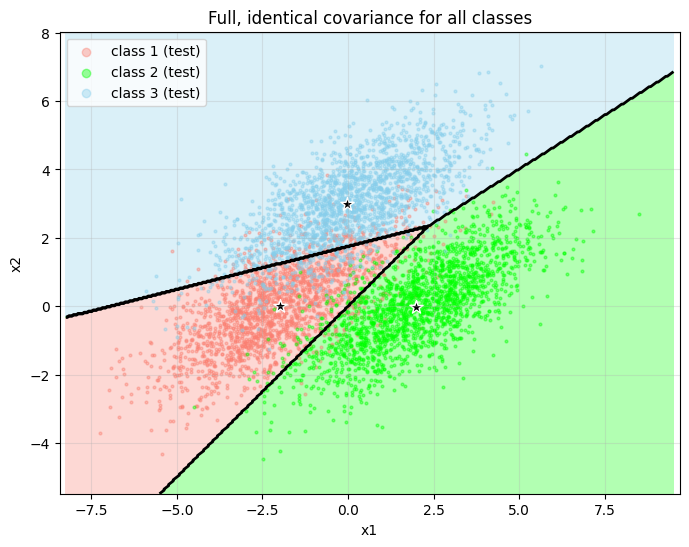
\includegraphics[width=\textwidth]{case3.png}
  \caption{Case 3: Full shared}
\end{subfigure}
\caption{Bayes decision boundaries and test data for identical covariance cases.}
\label{fig:identical}
\end{figure}

\begin{figure}[ht]
\centering
\begin{subfigure}{0.32\textwidth}
  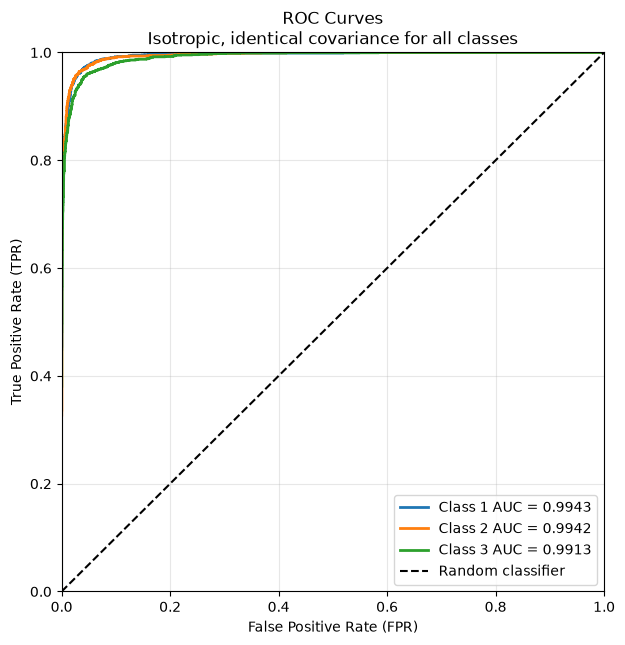
\includegraphics[width=\textwidth]{case1_roc.png}
  \caption{Case 1: ROC curves}
\end{subfigure}\hfill
\begin{subfigure}{0.32\textwidth}
  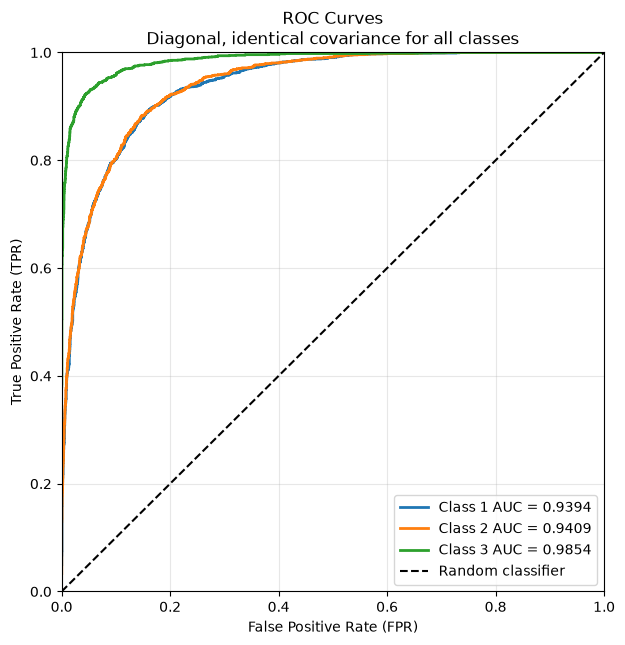
\includegraphics[width=\textwidth]{case2_roc.png}
  \caption{Case 2: ROC curves}
\end{subfigure}\hfill
\begin{subfigure}{0.32\textwidth}
  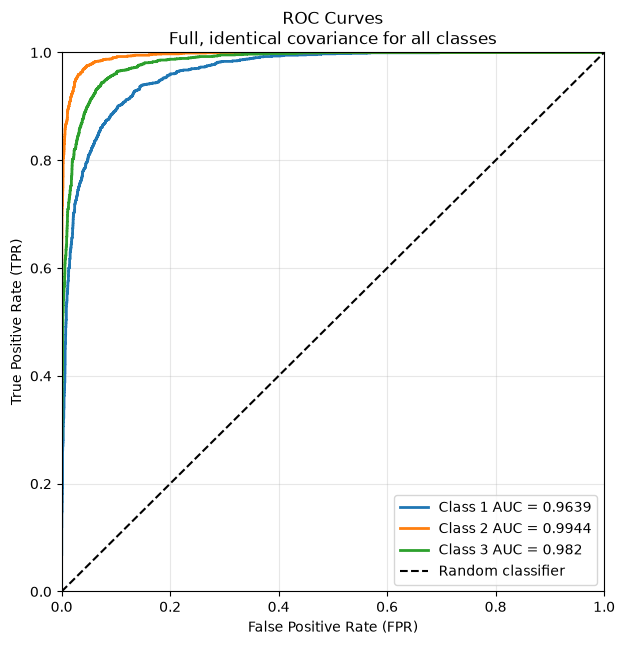
\includegraphics[width=\textwidth]{case3_roc.png}
  \caption{Case 3: ROC curves}
\end{subfigure}
\caption{One-vs-rest ROC curves for identical covariance cases.}
\label{fig:identical_roc}
\end{figure}

\subsubsection{Case 1: Isotropic, Identical Covariance ($\Sigma=\mathbf{I}$)}
\begin{itemize}
  \item \textbf{Target Covariance:} $\Sigma_1=\Sigma_2=\Sigma_3=\begin{bmatrix}1.0&0.0\\0.0&1.0\end{bmatrix}$.
  \item \textbf{Estimated Parameters:} $\hat{\mu}_1=[-1.99,-0.00]^T$, $\hat{\mu}_2=[2.00,-0.01]^T$, $\hat{\mu}_3=[-0.01,2.99]^T$. Common $\hat{\Sigma}=\begin{bmatrix}0.999&0.000\\0.000&0.999\end{bmatrix}$. Estimated priors $\hat{P}=[0.333,0.333,0.333]$.
  \item \textbf{Test Accuracy:} 94.55\%.
  \item \textbf{ROC AUC:} Class 1: 0.9943, Class 2: 0.9942, Class 3: 0.9913.
\end{itemize}
\textbf{Observations:}
\begin{itemize}
  \item Decision boundaries are perpendicular bisectors between class means.
  \item With equal spherical variance, classification is equivalent to nearest-centroid classification under Euclidean distance.
  \item High AUC ($>0.99$) across all classes confirms minimal overlap and near-ideal class ranking (Table~\ref{tab:c1}, Figure~\ref{fig:identical_roc}(a)).
\end{itemize}

\begin{table}[ht]
\centering
\begin{tabular}{cccc}
\toprule
\textbf{True Class} & \textbf{Pred Class 1} & \textbf{Pred Class 2} & \textbf{Pred Class 3}\\
\midrule
Class 1 & 1907 & 37 & 56\\
Class 2 & 36 & 1916 & 48\\
Class 3 & 63 & 75 & 1862\\
\bottomrule
\end{tabular}
\caption{Confusion matrix for Case 1 (Test Accuracy: 94.55\%).}
\label{tab:c1}
\end{table}

\subsubsection{Case 2: Diagonal, Identical Covariance ($\Sigma=\mathrm{diag}(4,1)$)}
\begin{itemize}
  \item \textbf{Target Covariance:} $\Sigma_1=\Sigma_2=\Sigma_3=\begin{bmatrix}4.0&0.0\\0.0&1.0\end{bmatrix}$.
  \item \textbf{Estimated Parameters:} $\hat{\mu}_1=[-2.04,0.02]^T$, $\hat{\mu}_2=[2.02,-0.00]^T$, $\hat{\mu}_3=[-0.00,2.98]^T$. Common $\hat{\Sigma}=\begin{bmatrix}4.025&0.000\\0.000&1.014\end{bmatrix}$.
  \item \textbf{Test Accuracy:} 84.70\%.
  \item \textbf{ROC AUC:} Class 1: 0.9394, Class 2: 0.9409, Class 3: 0.9854.
\end{itemize}
\textbf{Observations:}
\begin{itemize}
  \item Horizontal stretching ($\sigma_{x_1}^2=4.0$) creates significant overlap between Class 1 and Class 2, reducing their respective AUCs to $\approx 0.94$ (Figure~\ref{fig:identical_roc}(b)).
  \item Class 3 remains distinct along the vertical axis, retaining a higher AUC of 0.9854 (Table~\ref{tab:c2}).
\end{itemize}

\begin{table}[ht]
\centering
\begin{tabular}{cccc}
\toprule
\textbf{True Class} & \textbf{Pred Class 1} & \textbf{Pred Class 2} & \textbf{Pred Class 3}\\
\midrule
Class 1 & 1609 & 314 & 77\\
Class 2 & 300 & 1606 & 94\\
Class 3 & 99 & 70 & 1831\\
\bottomrule
\end{tabular}
\caption{Confusion matrix for Case 2 (Test Accuracy: 84.70\%).}
\label{tab:c2}
\end{table}

\subsubsection{Case 3: Full, Identical Covariance ($\Sigma=\begin{bmatrix}3.0&1.5\\1.5&1.5\end{bmatrix}$)}
\begin{itemize}
  \item \textbf{Target Covariance:} $\Sigma_1=\Sigma_2=\Sigma_3=\begin{bmatrix}3.0&1.5\\1.5&1.5\end{bmatrix}$.
  \item \textbf{Estimated Parameters:} $\hat{\mu}_1=[-2.00,0.01]^T$, $\hat{\mu}_2=[1.98,-0.02]^T$, $\hat{\mu}_3=[-0.02,2.99]^T$. Common $\hat{\Sigma}=\begin{bmatrix}2.983&1.502\\1.502&1.509\end{bmatrix}$.
  \item \textbf{Test Accuracy:} 89.77\%.
  \item \textbf{ROC AUC:} Class 1: 0.9639, Class 2: 0.9944, Class 3: 0.9820.
\end{itemize}
\textbf{Observations:}
\begin{itemize}
  \item Positive covariance ($\sigma_{12}=1.5$) tilts clusters diagonally, keeping decision boundaries as straight lines.
  \item Class 2 is oriented away from the elongation axis of Class 3, yielding only 4 misclassifications and the highest AUC of 0.9944 (Table~\ref{tab:c3}, Figure~\ref{fig:identical_roc}(c)).
\end{itemize}

\begin{table}[ht]
\centering
\begin{tabular}{cccc}
\toprule
\textbf{True Class} & \textbf{Pred Class 1} & \textbf{Pred Class 2} & \textbf{Pred Class 3}\\
\midrule
Class 1 & 1732 & 89 & 179\\
Class 2 & 113 & 1883 & 4\\
Class 3 & 197 & 8 & 1795\\
\bottomrule
\end{tabular}
\caption{Confusion matrix for Case 3 (Test Accuracy: 89.77\%).}
\label{tab:c3}
\end{table}

\subsection{Different Covariances Across Classes}
In Cases 4, 5, and 6, each class has a distinct covariance matrix. Because quadratic terms $x^T\hat{\Sigma}_k^{-1}x$ do not cancel, decision boundaries become curved quadratic contours (Figure~\ref{fig:different}). The corresponding one-vs-rest ROC curves are shown in Figure~\ref{fig:different_roc}.

\begin{figure}[ht]
\centering
\begin{subfigure}{0.32\textwidth}
  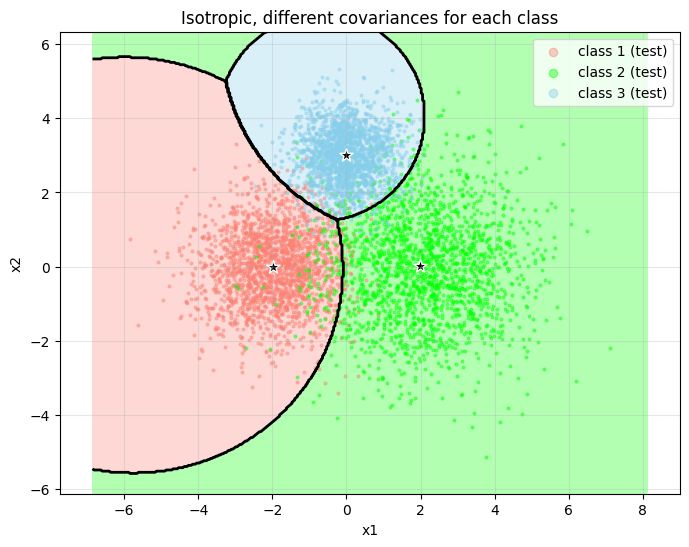
\includegraphics[width=\textwidth]{case4.png}
  \caption{Case 4: Isotropic unequal}
\end{subfigure}\hfill
\begin{subfigure}{0.32\textwidth}
  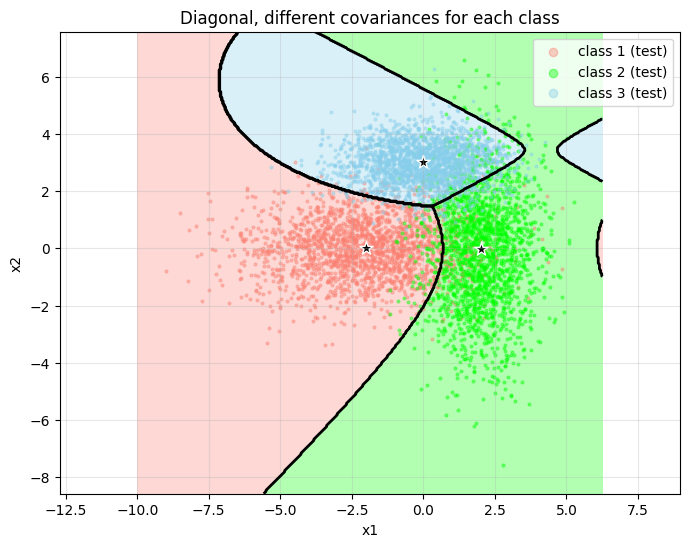
\includegraphics[width=\textwidth]{case5.png}
  \caption{Case 5: Diagonal unequal}
\end{subfigure}\hfill
\begin{subfigure}{0.32\textwidth}
  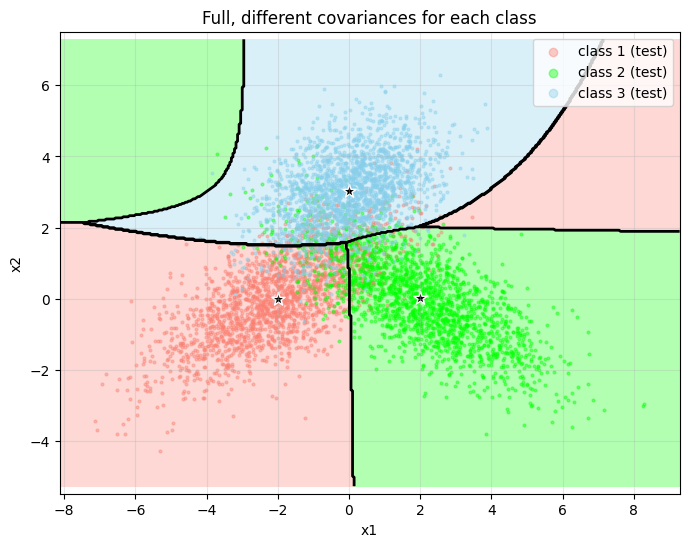
\includegraphics[width=\textwidth]{case6.png}
  \caption{Case 6: Full unequal}
\end{subfigure}
\caption{Bayes decision boundaries and test data for different covariance cases.}
\label{fig:different}
\end{figure}

\begin{figure}[ht]
\centering
\begin{subfigure}{0.32\textwidth}
  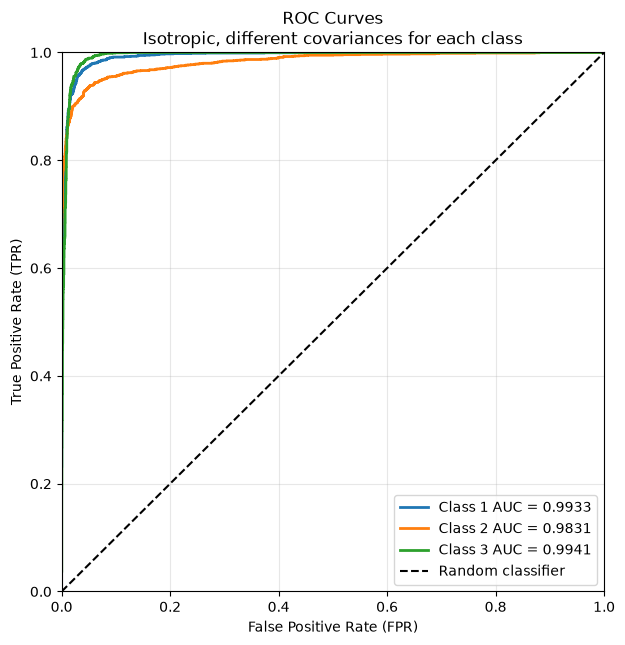
\includegraphics[width=\textwidth]{case4_roc.png}
  \caption{Case 4: ROC curves}
\end{subfigure}\hfill
\begin{subfigure}{0.32\textwidth}
  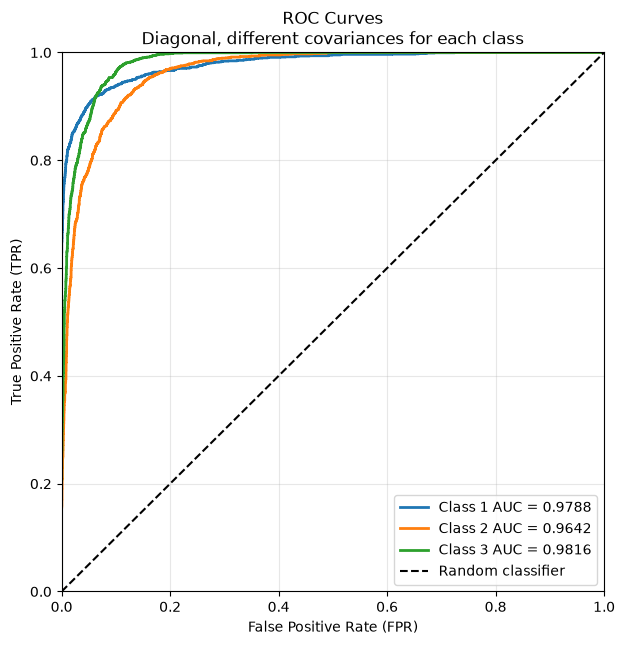
\includegraphics[width=\textwidth]{case5_roc.png}
  \caption{Case 5: ROC curves}
\end{subfigure}\hfill
\begin{subfigure}{0.32\textwidth}
  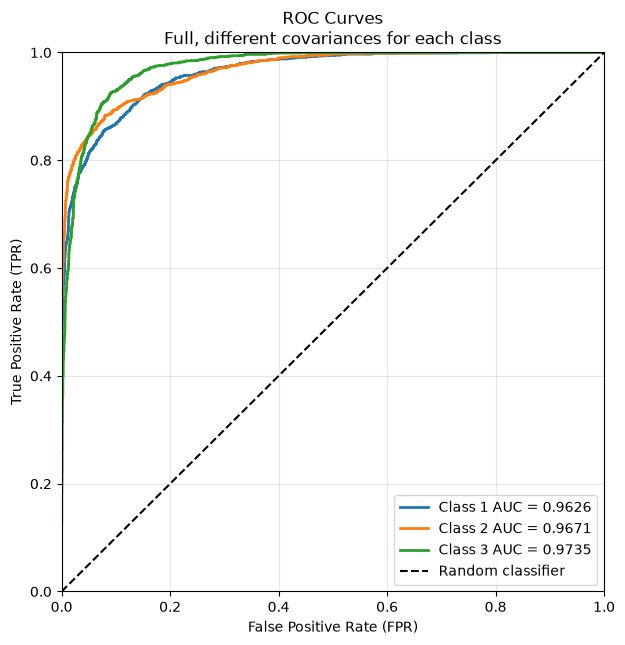
\includegraphics[width=\textwidth]{case6_roc.png}
  \caption{Case 6: ROC curves}
\end{subfigure}
\caption{One-vs-rest ROC curves for different covariance cases.}
\label{fig:different_roc}
\end{figure}

\subsubsection{Case 4: Isotropic, Different Covariances ($\sigma_1^2=1.0,\sigma_2^2=2.0,\sigma_3^2=0.5$)}
\begin{itemize}
  \item \textbf{Target Covariances:} $\Sigma_1=\mathbf{I}$, $\Sigma_2=2\mathbf{I}$, $\Sigma_3=0.5\mathbf{I}$.
  \item \textbf{Estimated Parameters:} $\hat{\mu}_1=[-2.00,-0.01]^T$, $\hat{\mu}_2=[1.99,0.02]^T$, $\hat{\mu}_3=[-0.01,3.00]^T$.\\
  $\hat{\Sigma}_1\approx\begin{bmatrix}1.011&0\\0&0.970\end{bmatrix}$,
  $\hat{\Sigma}_2\approx\begin{bmatrix}2.051&0\\0&1.998\end{bmatrix}$,
  $\hat{\Sigma}_3\approx\begin{bmatrix}0.511&0\\0&0.508\end{bmatrix}$.
  \item \textbf{Test Accuracy:} 93.95\%.
  \item \textbf{ROC AUC:} Class 1: 0.9933, Class 2: 0.9831, Class 3: 0.9941.
\end{itemize}
\textbf{Observations:}
\begin{itemize}
  \item Decision boundaries form circular arcs enclosing regions of smaller variance.
  \item Class 3 has the lowest variance ($\sigma_3^2=0.5$), resulting in a compact decision region and the highest AUC of 0.9941 (Table~\ref{tab:c4}, Figure~\ref{fig:different_roc}(a)).
\end{itemize}

\begin{table}[ht]
\centering
\begin{tabular}{cccc}
\toprule
\textbf{True Class} & \textbf{Pred Class 1} & \textbf{Pred Class 2} & \textbf{Pred Class 3}\\
\midrule
Class 1 & 1902 & 66 & 32\\
Class 2 & 100 & 1810 & 90\\
Class 3 & 17 & 42 & 1941\\
\bottomrule
\end{tabular}
\caption{Confusion matrix for Case 4 (Test Accuracy: 93.95\%).}
\label{tab:c4}
\end{table}

\subsubsection{Case 5: Diagonal, Different Covariances}
\begin{itemize}
  \item \textbf{Target Covariances:} $\Sigma_1=\mathrm{diag}(4,1)$, $\Sigma_2=\mathrm{diag}(1,4)$, $\Sigma_3=\mathrm{diag}(2,0.5)$.
  \item \textbf{Estimated Parameters:} $\hat{\mu}_1\approx[-1.99,-0.00]^T$, $\hat{\mu}_2\approx[2.02,-0.03]^T$, $\hat{\mu}_3\approx[-0.01,3.00]^T$.\\
  $\hat{\Sigma}_1\approx\mathrm{diag}(4.01,1.02)$, $\hat{\Sigma}_2\approx\mathrm{diag}(1.01,4.01)$, $\hat{\Sigma}_3\approx\mathrm{diag}(2.00,0.50)$.
  \item \textbf{Test Accuracy:} 88.55\%.
  \item \textbf{ROC AUC:} Class 1: 0.9788, Class 2: 0.9642, Class 3: 0.9816.
\end{itemize}
\textbf{Observations:}
\begin{itemize}
  \item Differing axis-aligned variances produce hyperbolic and parabolic boundary segments.
  \item Overlap between the horizontal spread of Class 1 and the vertical spread of Class 2 leads to moderate errors, while all class AUCs remain high ($>0.96$, Table~\ref{tab:c5}, Figure~\ref{fig:different_roc}(b)).
\end{itemize}

\begin{table}[ht]
\centering
\begin{tabular}{cccc}
\toprule
\textbf{True Class} & \textbf{Pred Class 1} & \textbf{Pred Class 2} & \textbf{Pred Class 3}\\
\midrule
Class 1 & 1746 & 192 & 62\\
Class 2 & 90 & 1680 & 230\\
Class 3 & 42 & 89 & 1869\\
\bottomrule
\end{tabular}
\caption{Confusion matrix for Case 5 (Test Accuracy: 88.55\%).}
\label{tab:c5}
\end{table}

\subsubsection{Case 6: Full, Different Covariances}
\begin{itemize}
  \item \textbf{Target Covariances:} $\Sigma_1=\begin{bmatrix}3.0&1.5\\1.5&1.5\end{bmatrix}$, $\Sigma_2=\begin{bmatrix}3.0&-1.5\\-1.5&1.5\end{bmatrix}$, $\Sigma_3=\begin{bmatrix}1.5&0.5\\0.5&1.0\end{bmatrix}$.
  \item \textbf{Estimated Parameters:} $\hat{\mu}_1\approx[-2.00,-0.00]^T$, $\hat{\mu}_2\approx[1.99,0.01]^T$, $\hat{\mu}_3\approx[-0.01,3.02]^T$.\\
  $\hat{\Sigma}_1\approx\begin{bmatrix}3.02&1.48\\1.48&1.50\end{bmatrix}$,
  $\hat{\Sigma}_2\approx\begin{bmatrix}2.97&-1.51\\-1.51&1.52\end{bmatrix}$,
  $\hat{\Sigma}_3\approx\begin{bmatrix}1.50&0.50\\0.50&1.00\end{bmatrix}$.
  \item \textbf{Test Accuracy:} 86.70\%.
  \item \textbf{ROC AUC:} Class 1: 0.9626, Class 2: 0.9671, Class 3: 0.9735.
\end{itemize}
\textbf{Observations:}
\begin{itemize}
  \item Opposite tilts of Class 1 and Class 2 generate rotated quadratic boundaries.
  \item Despite noticeable mutual overlap, ROC curves demonstrate balanced and robust discrimination across all classes ($\text{AUC} > 0.96$, Table~\ref{tab:c6}, Figure~\ref{fig:different_roc}(c)).
\end{itemize}

\begin{table}[ht]
\centering
\begin{tabular}{cccc}
\toprule
\textbf{True Class} & \textbf{Pred Class 1} & \textbf{Pred Class 2} & \textbf{Pred Class 3}\\
\midrule
Class 1 & 1655 & 164 & 181\\
Class 2 & 137 & 1706 & 157\\
Class 3 & 111 & 59 & 1830\\
\bottomrule
\end{tabular}
\caption{Confusion matrix for Case 6 (Test Accuracy: 86.70\%).}
\label{tab:c6}
\end{table}

\subsection{Real-World Dataset Classification (Part 2)}
The real-world dataset consists of 1,050 training points (350 per class) and 300 test points (100 per class). Class parameters were estimated using MLE with full, class-specific covariance matrices.

\begin{itemize}
  \item \textbf{Estimated Priors:} $\hat{P}(\omega_1)=\hat{P}(\omega_2)=\hat{P}(\omega_3)=0.333$.
  \item \textbf{Estimated Parameters:}
  \begin{itemize}
    \item Class 1: $\hat{\mu}_1=[583.79, 1441.97]^T$, $\hat{\Sigma}_1=\begin{bmatrix}25117.8&4183.8\\4183.8&59211.7\end{bmatrix}$, correlation $\rho_1=0.108$.
    \item Class 2: $\hat{\mu}_2=[339.33, 2036.19]^T$, $\hat{\Sigma}_2=\begin{bmatrix}6391.2&-5902.4\\-5902.4&42093.3\end{bmatrix}$, correlation $\rho_2=-0.360$.
    \item Class 3: $\hat{\mu}_3=[476.91, 1037.76]^T$, $\hat{\Sigma}_3=\begin{bmatrix}20943.3&25289.7\\25289.7&82273.9\end{bmatrix}$, correlation $\rho_3=0.609$.
  \end{itemize}
  \item \textbf{Test Accuracy:} 89.00\%.
  \item \textbf{ROC AUC:} Class 1: 0.9162, Class 2: 0.9886, Class 3: 0.9481.
\end{itemize}

\begin{figure}[ht]
\centering
\begin{subfigure}{0.48\textwidth}
  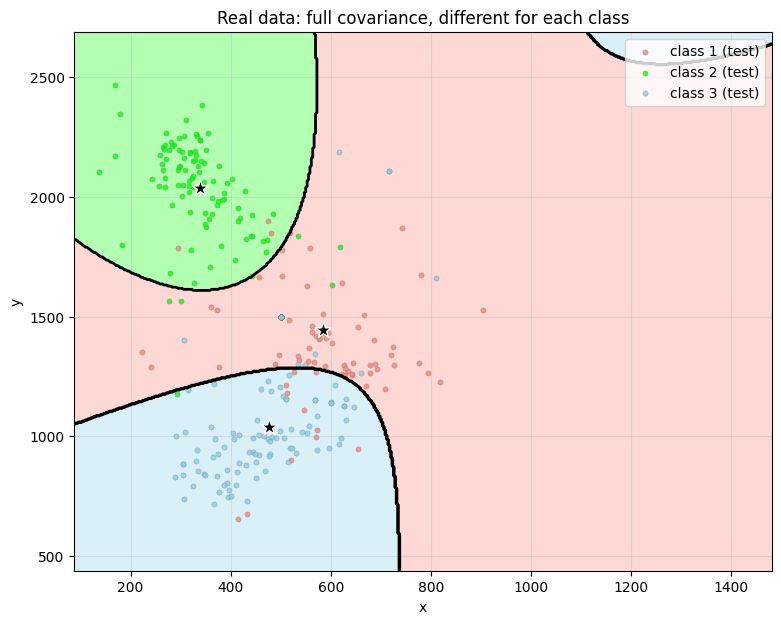
\includegraphics[width=\textwidth]{part2_decision_boundary.png}
  \caption{Decision boundaries and test data}
\end{subfigure}\hfill
\begin{subfigure}{0.48\textwidth}
  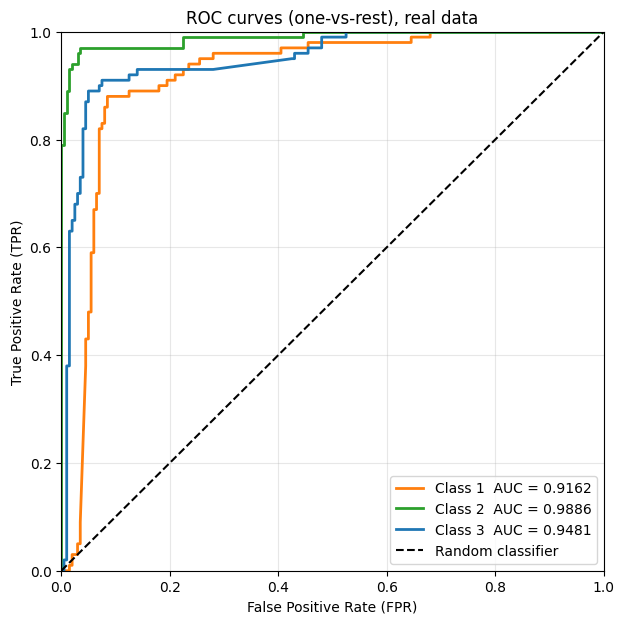
\includegraphics[width=\textwidth]{part_2_roc.png}
  \caption{One-vs-rest ROC curves}
\end{subfigure}\\[6pt]
\begin{subfigure}{0.96\textwidth}
  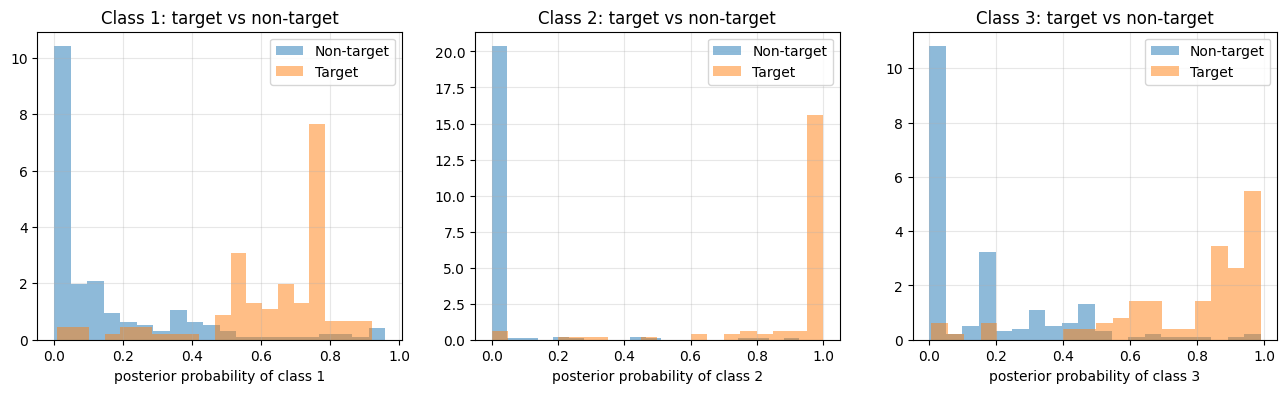
\includegraphics[width=\textwidth]{Target_nonTarget_distribution.png}
  \caption{Target vs. non-target posterior probability distributions}
\end{subfigure}
\caption{Classification results, ROC curves, and posterior distributions for the real-world dataset (Part 2).}
\label{fig:part2}
\end{figure}

\begin{table}[ht]
\centering
\begin{tabular}{cccc}
\toprule
\textbf{True Class} & \textbf{Pred Class 1} & \textbf{Pred Class 2} & \textbf{Pred Class 3}\\
\midrule
Class 1 & 85 & 4 & 11\\
Class 2 & 6 & 93 & 1\\
Class 3 & 11 & 0 & 89\\
\bottomrule
\end{tabular}
\caption{Confusion matrix for Part 2 real-world data (Test Accuracy: 89.00\%).}
\label{tab:c_real}
\end{table}

\textbf{Observations and Plot Findings:}
\begin{itemize}
  \item \textbf{Decision Boundaries:} Differing variances and orientations across classes produce curved quadratic decision boundaries. Class 2 is situated at the top and clearly partitioned, while Classes 1 and 3 share a curved vertical boundary (Figure~\ref{fig:part2}(a)).
  \item \textbf{Target vs. Non-Target Distributions:} In Figure~\ref{fig:part2}(c), Class 2 shows clear separation with posterior probabilities tightly concentrated near 1.0 for targets and near 0.0 for non-targets. Classes 1 and 3 display slight score overlap around intermediate probabilities, corresponding to the 11 mutual misclassifications in Table~\ref{tab:c_real}.
  \item \textbf{ROC Curves:} Figure~\ref{fig:part2}(b) shows strong discrimination across all classes. Class 2 achieves the highest AUC of 0.9886, followed by Class 3 (0.9481) and Class 1 (0.9162).
\end{itemize}

\subsection{Summary of Results Across All Cases}
Table~\ref{tab:summary} summarizes the classification performance, boundary shapes, and ROC AUC scores across all synthetic cases and the real-world dataset.

\begin{table}[ht]
\centering
\small
\begin{tabular}{@{}clllcc@{}}
\toprule
\textbf{Case} & \textbf{Covariance Structure} & \textbf{Covariance Equality} & \textbf{Boundary Shape} & \textbf{Test Acc.} & \textbf{ROC AUC ($C_1 / C_2 / C_3$)}\\
\midrule
1 & Isotropic ($\sigma^2 I$) & Identical ($\Sigma_i=\Sigma$) & Linear (straight lines) & 94.55\% & 0.994 / 0.994 / 0.991\\
2 & Diagonal ($\mathrm{diag}(\sigma_1^2,\sigma_2^2)$) & Identical ($\Sigma_i=\Sigma$) & Linear (slanted lines) & 84.70\% & 0.939 / 0.941 / 0.985\\
3 & Full ($\Sigma$) & Identical ($\Sigma_i=\Sigma$) & Linear (rotated lines) & 89.77\% & 0.964 / 0.994 / 0.982\\
4 & Isotropic ($\sigma_i^2 I$) & Different ($\Sigma_i\neq\Sigma_j$) & Quadratic (circular arcs) & 93.95\% & 0.993 / 0.983 / 0.994\\
5 & Diagonal ($\mathrm{diag}(\sigma_{i1}^2,\sigma_{i2}^2)$) & Different ($\Sigma_i\neq\Sigma_j$) & Quadratic (axis-aligned curves) & 88.55\% & 0.979 / 0.964 / 0.982\\
6 & Full ($\Sigma_i$) & Different ($\Sigma_i\neq\Sigma_j$) & Quadratic (rotated curves) & 86.70\% & 0.963 / 0.967 / 0.974\\
\midrule
Part 2 & Full ($\Sigma_i$) & Different ($\Sigma_i\neq\Sigma_j$) & Quadratic (curved) & 89.00\% & 0.916 / 0.989 / 0.948\\
\bottomrule
\end{tabular}
\caption{Comparison of classification results and ROC AUC values across all experiments.}
\label{tab:summary}
\end{table}

\section{Conclusion}
In this assignment, Maximum Likelihood Estimation was used to estimate Gaussian parameters for six synthetic covariance configurations and a real-world dataset. Classifying test samples under the Bayes decision rule confirmed that identical covariances produce linear decision boundaries, whereas unequal covariances produce quadratic boundaries. Confusion matrices, posterior score distributions, and one-vs-rest ROC curves demonstrated strong classification and ranking performance across all configurations, with AUC values exceeding 0.91 in every experiment.

\end{document}
